\documentclass[tikz, border=5pt]{standalone}

\newcommand{\threshdraw}[3]{%
  \draw[->] (#1) --
    node[pos=0.5] {\tikz \fill (0,0) -- (0.2,0.3) -- (-0.2,0.3) -- cycle;}
    node[pos=0.5, xshift=15pt] {\tiny $\tau_{#3}$}
  (#2);
}

\usepackage{tikz}
\usetikzlibrary{
  arrows.meta,
  calc,
  positioning,
  shapes.geometric,
  shadows.blur,
  bending,
  decorations.markings
}

\begin{document}

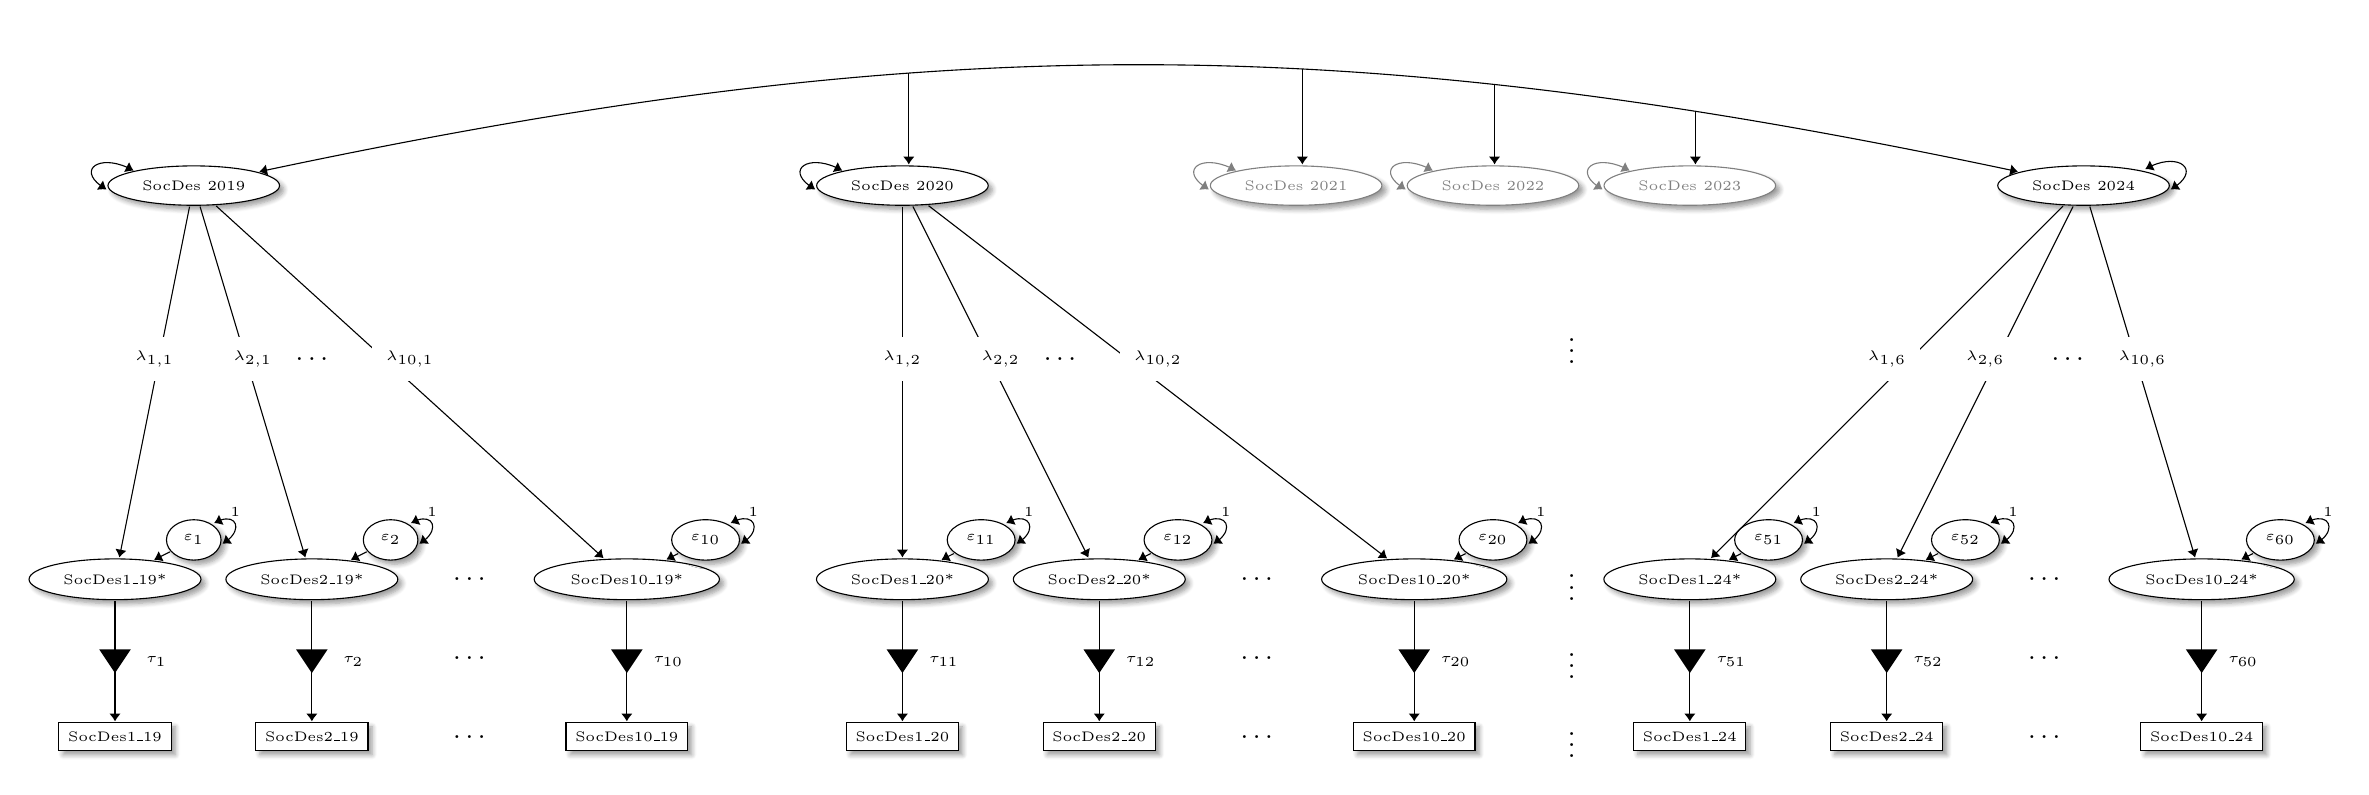
\begin{tikzpicture}

\tikzset{
  threshold/.style n args={1}{
  postaction={
    decorate,
    decoration={
      markings,
      mark=at position 0.5 with {
        \fill (0,0) -- (0.2,0.3) -- (-0.2,0.3) -- cycle;
        \node[xshift=15pt] {\tiny $#1$};
      }
    }
  }
},  
  socdesyear/.style={
    draw,
    ellipse,
    fill=white,
    % minimum width=2.6cm,
    % minimum height=0.9cm,
    align=center,
    font = \tiny,
    blur shadow={shadow xshift=1.5pt, shadow yshift=-1.5pt, shadow blur steps=6}
  },
    socdesyeargrey/.style={
    draw=gray,
    ellipse,
    fill=white,
    text=gray,
    % minimum width=2.6cm,
    % minimum height=0.9cm,
    align=center,
    font = \tiny,
  blur shadow={shadow xshift=1.5pt, shadow yshift=-1.5pt, shadow blur steps=6}
},  
  observ/.style={
    draw,
    rectangle,
    fill=white,
    % minimum width=2.8cm,
    % minimum height=1.1cm,
    align=center,
    font=\tiny,
    blur shadow={shadow xshift=1.5pt, shadow yshift=-1.5pt, shadow blur steps=6}
  },
  epsil/.style={
  draw,
  ellipse,
  fill=white,
  align=center,
  font=\tiny,
  blur shadow={shadow xshift=1.5pt, shadow yshift=-1.5pt, shadow blur steps=6}
  },
  >={Latex[length=1mm, width=1.5mm]},
  line width=1pt
}

% NODES ----------------------------------------------------------

% Nodes Latent Annual Variables
\node[socdesyear]     (sd2019) at (1,  7) {SocDes 2019};
\node[socdesyear]     (sd2020) at (10, 7) {SocDes 2020};
\node[socdesyeargrey] (sd2021) at (15, 7) {SocDes 2021};
\node[socdesyeargrey] (sd2022) at (17.5, 7) {SocDes 2022};
\node[socdesyeargrey] (sd2023) at (20, 7) {SocDes 2023};
\node[socdesyear]     (sd2024) at (25, 7) {SocDes 2024};

% Nodes SocDes Star (use the same style of `socdesyear`) + Dots
\node[socdesyear] (y1star)   at (0   , 2)   {SocDes1\_19*};
\node[socdesyear] (y2star)   at (2.5 , 2)   {SocDes2\_19*};
\node             (dots)     at (2.5 , 4.8) {$\dots$}; % dots for lambda
\node             (dots)     at (4.5 , 2)   {$\dots$}; % dots for ellipse
\node             (dots)     at (4.5 , 1)   {$\dots$}; % dots for tau
\node[socdesyear] (y10star)  at (6.5 , 2)   {SocDes10\_19*};

\node[socdesyear] (y11star)  at (10,   2)   {SocDes1\_20*};
\node[socdesyear] (y12star)  at (12.5, 2)   {SocDes2\_20*};
\node             (dots)     at (12,   4.8) {$\dots$}; % dots for lambda
\node             (dots)     at (14.5, 2)   {$\dots$}; % dots for ellipse
\node             (dots)     at (14.5, 1)   {$\dots$}; % dots for tau
\node[socdesyear] (y20star)  at (16.5, 2)   {SocDes10\_20*};

\node             (dots)     at (18.5, 5)   {$\vdots$}; % all vertical dots
\node             (dots)     at (18.5, 2)   {$\vdots$};
\node             (dots)     at (18.5, 1)   {$\vdots$};
\node             (dots)     at (18.5, 0)   {$\vdots$};

\node[socdesyear] (y51star)  at (20  , 2)   {SocDes1\_24*};
\node[socdesyear] (y52star)  at (22.5, 2)   {SocDes2\_24*};
\node             (dots)     at (24.8, 4.8)   {$\dots$}; % dots for lambda
\node             (dots)     at (24.5, 2)   {$\dots$}; % dots for ellipse
\node             (dots)     at (24.5, 1)   {$\dots$}; % dots for tau
\node[socdesyear] (y60star)  at (26.5, 2)   {SocDes10\_24*};


% Nodes categorical observed variables
\node[observ] (y1)   at (0,    0) {SocDes1\_19};
\node[observ] (y2)   at (2.5,  0) {SocDes2\_19};
\node         (dots) at (4.5,  0) {$\dots$};
\node[observ] (y10)  at (6.5,  0) {SocDes10\_19};

\node[observ] (y11)   at (10,  0) {SocDes1\_20};
\node[observ] (y12)   at (12.5,0) {SocDes2\_20};
\node         (dots)  at  (14.5,0) {$\dots$};
\node[observ] (y20)   at  (16.5,0) {SocDes10\_20};

\node[observ] (y51)   at (20,  0) {SocDes1\_24};
\node[observ] (y52)   at (22.5,0) {SocDes2\_24};
\node         (dots)  at (24.5,0) {$\dots$};
\node[observ] (y60)   at (26.5,0) {SocDes10\_24};



% Nodes epsilon
\node[epsil] (e1)  at (1,   2.5)   {$\varepsilon_{1}$};
\node[epsil] (e2)  at (3.5, 2.5)   {$\varepsilon_{2}$};
\node[epsil] (e10) at (7.5, 2.5)   {$\varepsilon_{10}$};

\node[epsil] (e11)  at (11,   2.5)   {$\varepsilon_{11}$};
\node[epsil] (e12)  at (13.5, 2.5)   {$\varepsilon_{12}$};
\node[epsil] (e20) at  (17.5, 2.5)   {$\varepsilon_{20}$};

\node[epsil] (e51)  at (21,   2.5)   {$\varepsilon_{51}$};
\node[epsil] (e52)  at (23.5, 2.5)   {$\varepsilon_{52}$};
\node[epsil] (e60) at  (27.5, 2.5)   {$\varepsilon_{60}$};


% DRAWS ---------------------------------------------------------

% Draws latent categorical + triangle
\threshdraw{y1star}{y1}{1}
\threshdraw{y2star}{y2}{2}
\threshdraw{y10star}{y10}{10}

\threshdraw{y11star}{y11}{11}
\threshdraw{y12star}{y12}{12}
\threshdraw{y20star}{y20}{20}

\threshdraw{y51star}{y51}{51}
\threshdraw{y52star}{y52}{52}
\threshdraw{y60star}{y60}{60}


% Draw epsilon
\draw[->] (e1) -- (y1star);
\draw[->] (e2) -- (y2star);
\draw[->] (e10) -- (y10star);

\draw[->] (e11) -- (y11star);
\draw[->] (e12) -- (y12star);
\draw[->] (e20) -- (y20star);

\draw[->] (e51) -- (y51star);
\draw[->] (e52) -- (y52star);
\draw[->] (e60) -- (y60star);


% Draw lambda
\draw[->] (sd2019) -- node[midway, above, font=\tiny, fill=white, inner sep=5pt] {$\lambda_{1,1}$}  (y1star);
\draw[->] (sd2019) -- node[midway, above, font=\tiny, fill=white, inner sep=5pt] {$\lambda_{2,1}$}  (y2star);
\draw[->] (sd2019) -- node[midway, above, font=\tiny, fill=white, inner sep=5pt] {$\lambda_{10,1}$} (y10star);

\draw[->] (sd2020) -- node[midway, above, font=\tiny, fill=white, inner sep=5pt] {$\lambda_{1,2}$}  (y11star);
\draw[->] (sd2020) -- node[midway, above, font=\tiny, fill=white, inner sep=5pt] {$\lambda_{2,2}$}  (y12star);
\draw[->] (sd2020) -- node[midway, above, font=\tiny, fill=white, inner sep=5pt] {$\lambda_{10,2}$} (y20star);

\draw[->] (sd2024) -- node[midway, above, font=\tiny, fill=white, inner sep=5pt] {$\lambda_{1,6}$}  (y51star);
\draw[->] (sd2024) -- node[midway, above, font=\tiny, fill=white, inner sep=5pt] {$\lambda_{2,6}$}  (y52star);
\draw[->] (sd2024) -- node[midway, above, font=\tiny, fill=white, inner sep=5pt] {$\lambda_{10,6}$} (y60star);


% Arrows Covariances
\draw[<->] (sd2019) to[bend left=12]
  coordinate[pos=0.36] (p1)
  coordinate[pos=0.60] (p2)
  coordinate[pos=0.715] (p3)
  coordinate[pos=0.83] (p4)
(sd2024);

\draw[->] (p1) -- ($(p1 |- sd2020.north)$);
\draw[->] (p2) -- ($(p2 |- sd2021.north)$);
\draw[->] (p3) -- ($(p3 |- sd2022.north)$);
\draw[->] (p4) -- ($(p4 |- sd2023.north)$);


% Variances of Soc Des Annual Latent Variables -------------------------------------------------
\draw[<->]
($(sd2019.north west)+(0.02,0.00)$)
to[out=150, in=150, looseness=3]
($(sd2019.west)+(0,-0.05)$);

\draw[<->]
($(sd2020.north west)+(0.02,0.00)$)
to[out=150, in=150, looseness=3]
($(sd2020.west)+(0,-0.05)$);

\draw[<->, draw=gray]
($(sd2021.north west)+(0.02,0.00)$)
to[out=150, in=150, looseness=3]
($(sd2021.west)+(0,-0.05)$);

\draw[<->, draw=gray]
($(sd2022.north west)+(0.02,0.00)$)
to[out=150, in=150, looseness=3]
($(sd2022.west)+(0,-0.05)$);

\draw[<->, draw=gray]
($(sd2023.north west)+(0.02,0.00)$)
to[out=150, in=150, looseness=3]
($(sd2023.west)+(0,-0.05)$);

\draw[<->]
($(sd2024.north east)+(0.00,0.02)$)
to[out=30, in=30, looseness=3]
($(sd2024.east)+(0,-0.05)$);

% Variances of epsilon ----------------------

%% Variance of epsilon 1
\draw[<->]
($(e1.north east)+(0.00,0.02)$)
to[out=30, in=30, looseness=3]
node[pos=0.5, above, font=\tiny, inner sep=2pt] {$1$}
($(e1.east)+(0,-0.05)$);

%% Variance of epsilon 2
\draw[<->]
($(e2.north east)+(0.00,0.02)$)
to[out=30, in=30, looseness=3]
node[pos=0.5, above, font=\tiny, inner sep=2pt] {$1$}
($(e2.east)+(0,-0.05)$);

%% Variance of epsilon 10
\draw[<->]
($(e10.north east)+(0.00,0.02)$)
to[out=30, in=30, looseness=3]
node[pos=0.5, above, font=\tiny, inner sep=2pt] {$1$}
($(e10.east)+(0,-0.05)$);

%% Variance of epsilon 11
\draw[<->]
($(e11.north east)+(0.00,0.02)$)
to[out=30, in=30, looseness=3]
node[pos=0.5, above, font=\tiny, inner sep=2pt] {$1$}
($(e11.east)+(0,-0.05)$);

%% Variance of epsilon 12
\draw[<->]
($(e12.north east)+(0.00,0.02)$)
to[out=30, in=30, looseness=3]
node[pos=0.5, above, font=\tiny, inner sep=2pt] {$1$}
($(e12.east)+(0,-0.05)$);

%% Variance of epsilon 20
\draw[<->]
($(e20.north east)+(0.00,0.02)$)
to[out=30, in=30, looseness=3]
node[pos=0.5, above, font=\tiny, inner sep=2pt] {$1$}
($(e20.east)+(0,-0.05)$);

%% Variance of epsilon 51
\draw[<->]
($(e51.north east)+(0.00,0.02)$)
to[out=30, in=30, looseness=3]
node[pos=0.5, above, font=\tiny, inner sep=2pt] {$1$}
($(e51.east)+(0,-0.05)$);

%% Variance of epsilon 52
\draw[<->]
($(e52.north east)+(0.00,0.02)$)
to[out=30, in=30, looseness=3]
node[pos=0.5, above, font=\tiny, inner sep=2pt] {$1$}
($(e52.east)+(0,-0.05)$);

%% Variance of epsilon 60
\draw[<->]
($(e60.north east)+(0.00,0.02)$)
to[out=30, in=30, looseness=3]
node[pos=0.5, above, font=\tiny, inner sep=2pt] {$1$}
($(e60.east)+(0,-0.05)$);

\end{tikzpicture}

\end{document}